
\begin{frame}{Control Structure}
	We elect for a cascaded control structure with optimal central control and local PI control.
	\begin{figure}[h!]
		\centering
		\resizebox{\columnwidth}{!}{
				\begin{tikzpicture}[auto, node distance=2.5cm,>=latex']
	% ========================== Nodes ============================
	% Nodes in upper vertical line
	\node [input, name=rinput] (rinput) {};
	\node [sum, right of=rinput] (sum1) {};
	\node [block, right of=sum1, node distance = 1.5cm] (LQR) {LQR};
	\node [sum, right of=LQR, node distance =
	1.5cm] (sum2) {};
	\node [block, right of=sum2, node distance = 1.5cm] (PID){PID};
	\node [block, right of=PID, align=center] (Fast){Fast\\Dynamics};
	\node [block, right of=Fast, node distance = 3cm, align=center] (Slow){Slow\\Dynamics};
	\node [output, right of=Slow] (output) {};
	
	% Nodes for inner feedback
	\node [tmp, right of=Fast, node distance = 1.5cm] (tmp0){};
	\node [tmp, below of=tmp0, node distance = 1.5cm] (tmp1){};
	\node [tmp, below of=sum2, node distance = 1.5cm] (tmp2){};
	
	% Nodes for outer feedback
	\node [tmp, right of=Slow, node distance = 1.5cm] (tmp10){};
	\node [tmp, below of=tmp10,node distance = 2.5cm] (tmp11){};
	\node [tmp, below of=sum1, node distance = 2.5cm] (tmp12){};
	
	% Nodes for Disturbance
	\node [tmp, above of=tmp0, node distance = 2.5cm] (tmp20){};
	\node [tmp, above of=tmp0, node distance = 2cm] (tmp21){};
	\node [tmp, above of=Fast, node distance = 2cm] (tmp22){};
	\node [tmp, above of=Slow, node distance = 2cm] (tmp23){};
	
	\draw[thick, dotted] ($(Fast.north west)+(-0.25, 0.25)$) rectangle  ($(Slow.south east)+(0.25, -0.25)$);
	\node[above of =tmp0, node distance =1.1cm](sys_txt) {System};
	
	% ========================== Lines ============================
	
	% Lines in upper vertical part of block diagram
	\draw [->] (rinput) -- node{$p_{ref}$} (sum1);
	\draw [->] (sum1) --node[name=z,anchor=north]{} (LQR);
	\draw [->] (LQR) -- node{$ q_{ref} $}(sum2);
	\draw [->] (sum2) -- (PID);
	\draw [->] (PID) -- node[pos=0.4]{$ \omega_{ref} $}(Fast);
	\draw [->] (Fast) -- node{$d_p$}(Slow);
	\draw [->] (Slow) -- node{$p_{\tau}$}(output);	
	
	% Lines for inner feedback
	\draw [-] (tmp0) -- (tmp1);
	\draw [-] (tmp1) -- (tmp2);
	\draw [->] (tmp2) -- node[pos=0.99]{$ - $}(sum2);
	
	
	% Lines for outer feedback
	\draw [-] (tmp10) -- (tmp11);
	\draw [-] (tmp11) -- (tmp12);
	\draw [->] (tmp12) -- node[pos=0.99]{$ - $}(sum1);
	
	
	% Lines for disturbance
	\draw [-] (tmp20)node[above, align=center]{Consumer \\ Disturbance} -- (tmp21);
	\draw [-] (tmp21) -- (tmp22);
	\draw [-] (tmp21) -- (tmp23);
	\draw [->] (tmp22) -- node[left, pos = 0.5]{$\Theta$}(Fast);
	\draw [->] (tmp23) -- node[pos = 0.5]{$ d_c $}(Slow);
	
	
\end{tikzpicture}
}
		\label{fig:tikzControlStrat}
	\end{figure}
\end{frame}

\begin{frame}{Control Structure}{The Root Locus Method}
	The root locus method needs a transfer function.\\
	Investigate decentralised control.\\
	\begin{figure}[h]
		\centering
		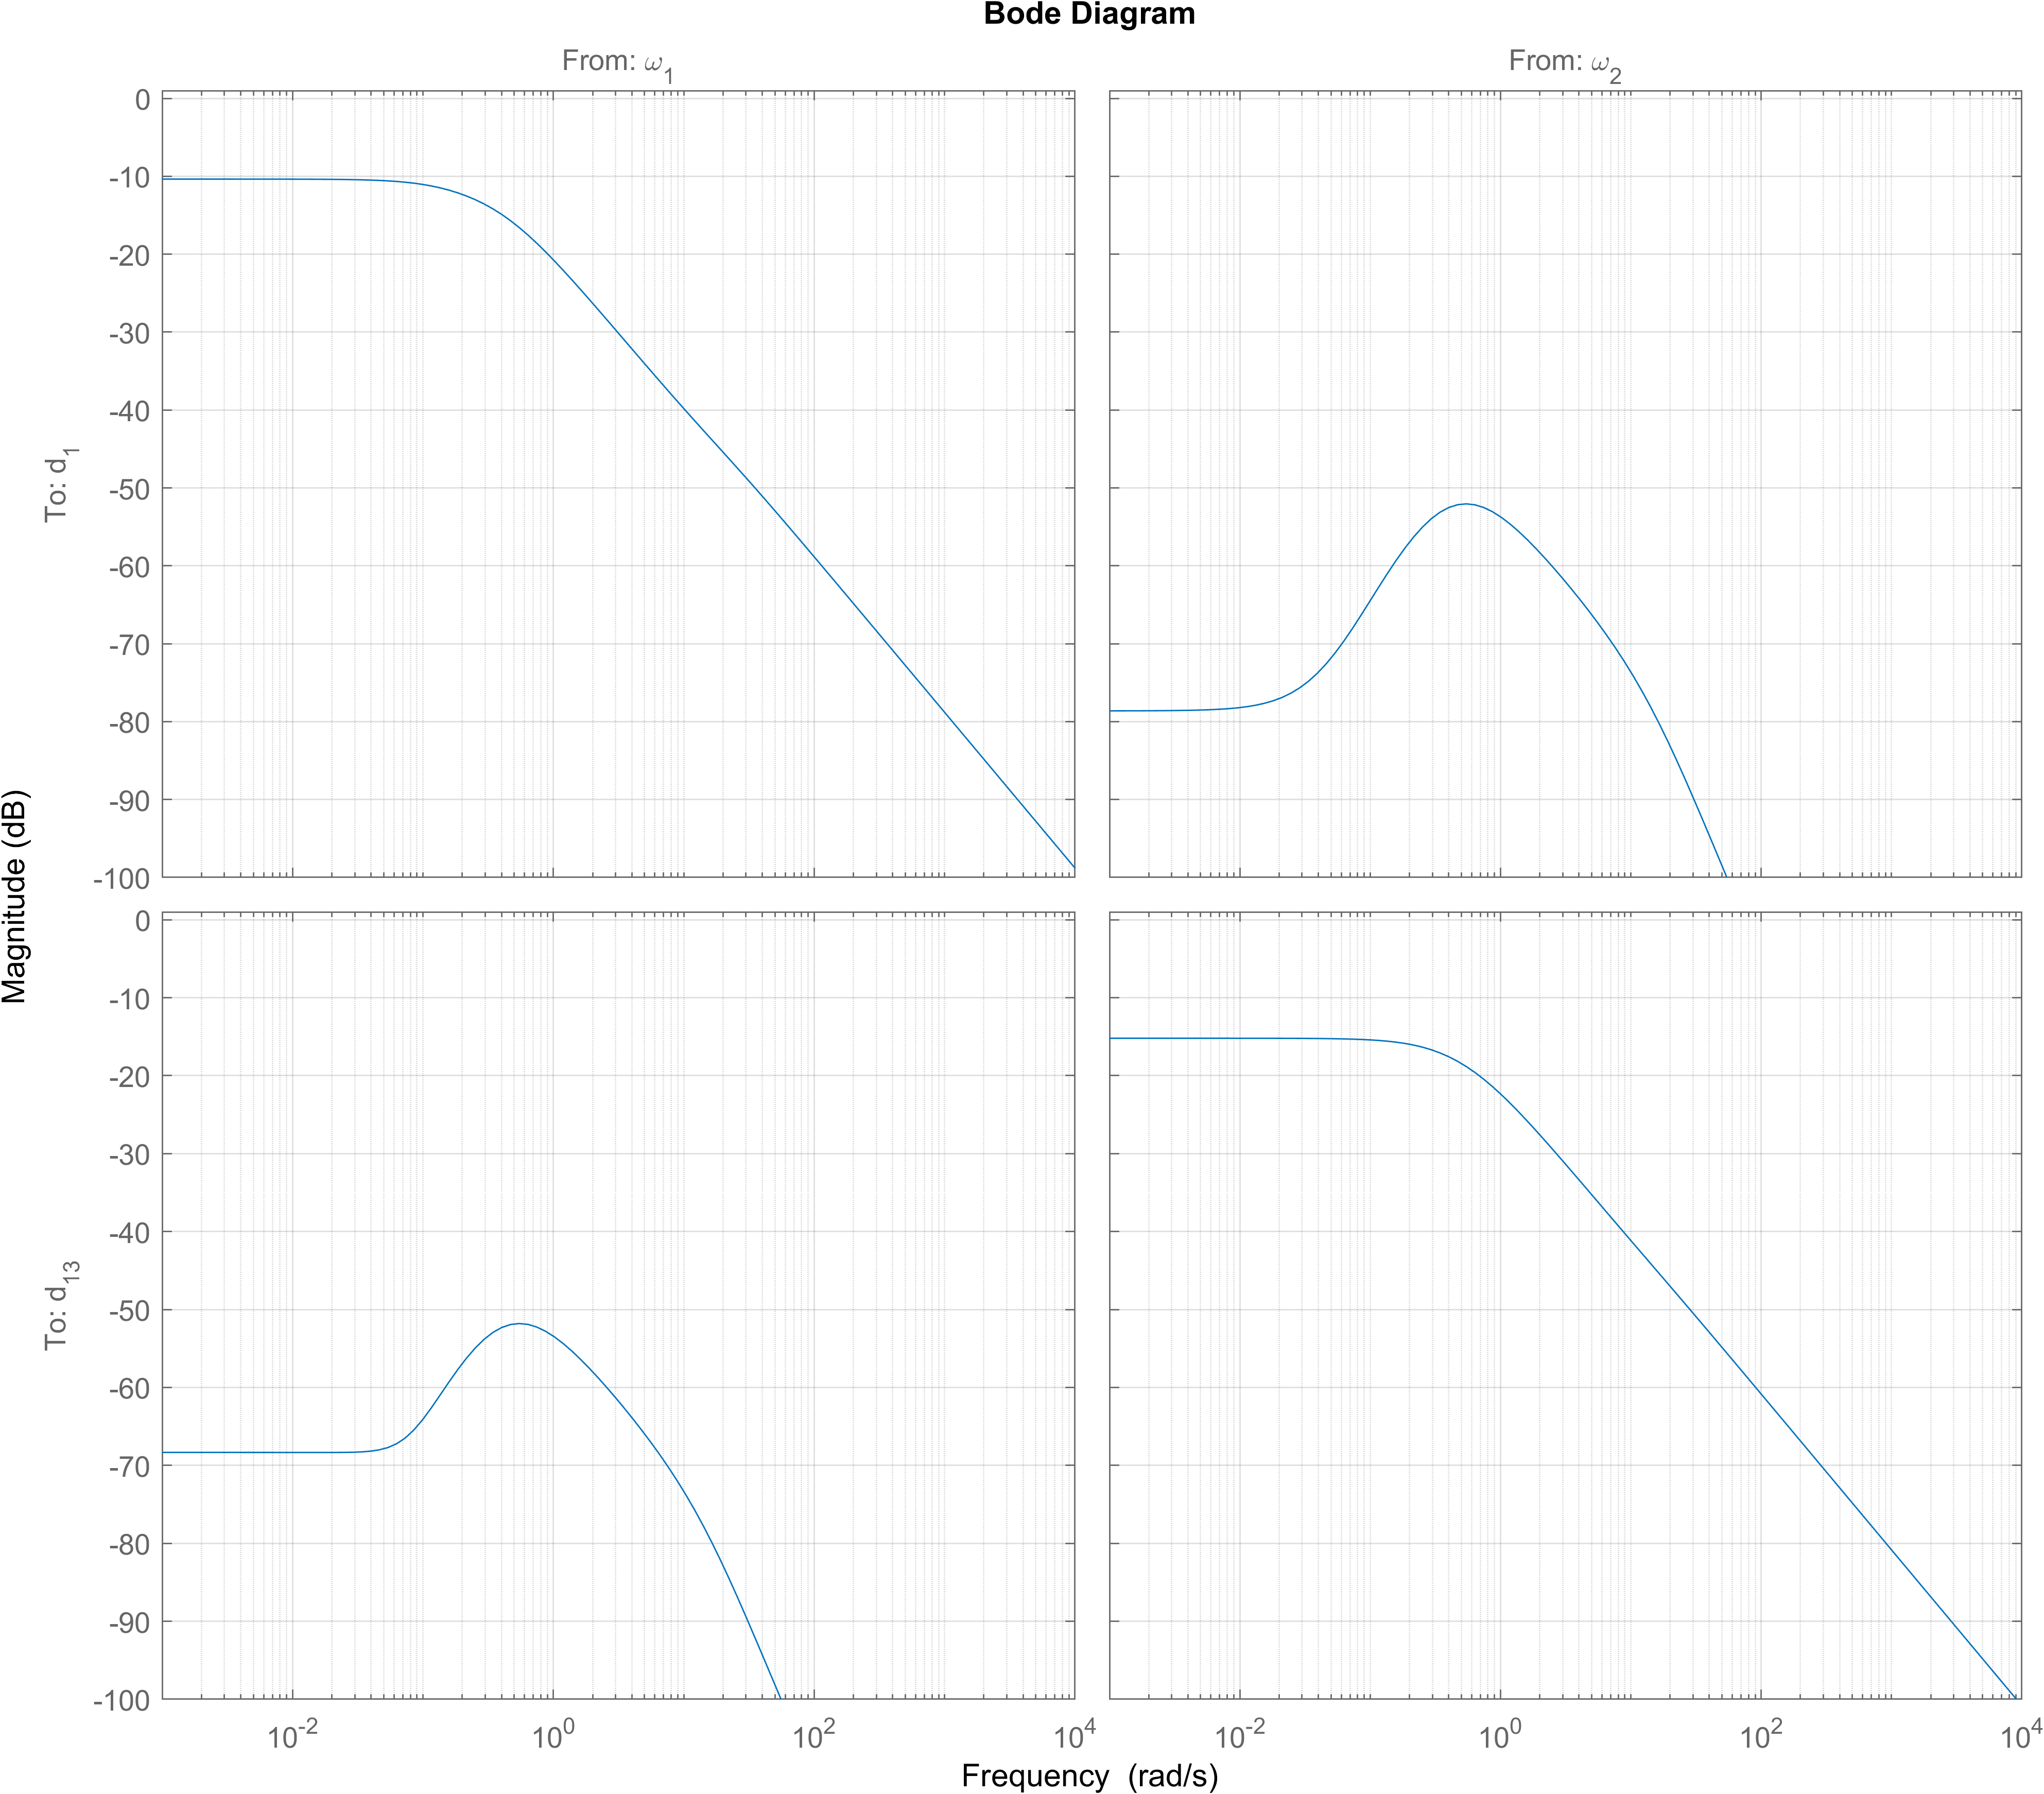
\includegraphics[height=5cm,width=0.5\linewidth]{Topics/ControlStructure/Graphics/PumpMagPlot.png}
		\label{fig:PumpMagPlot}
	\end{figure}
\end{frame}

\begin{frame}{Control Structure}{The Root Locus Method}
	Model order reduction.\\
	Padé approximation of delay.\\
	\begin{figure}[h]
		\centering
		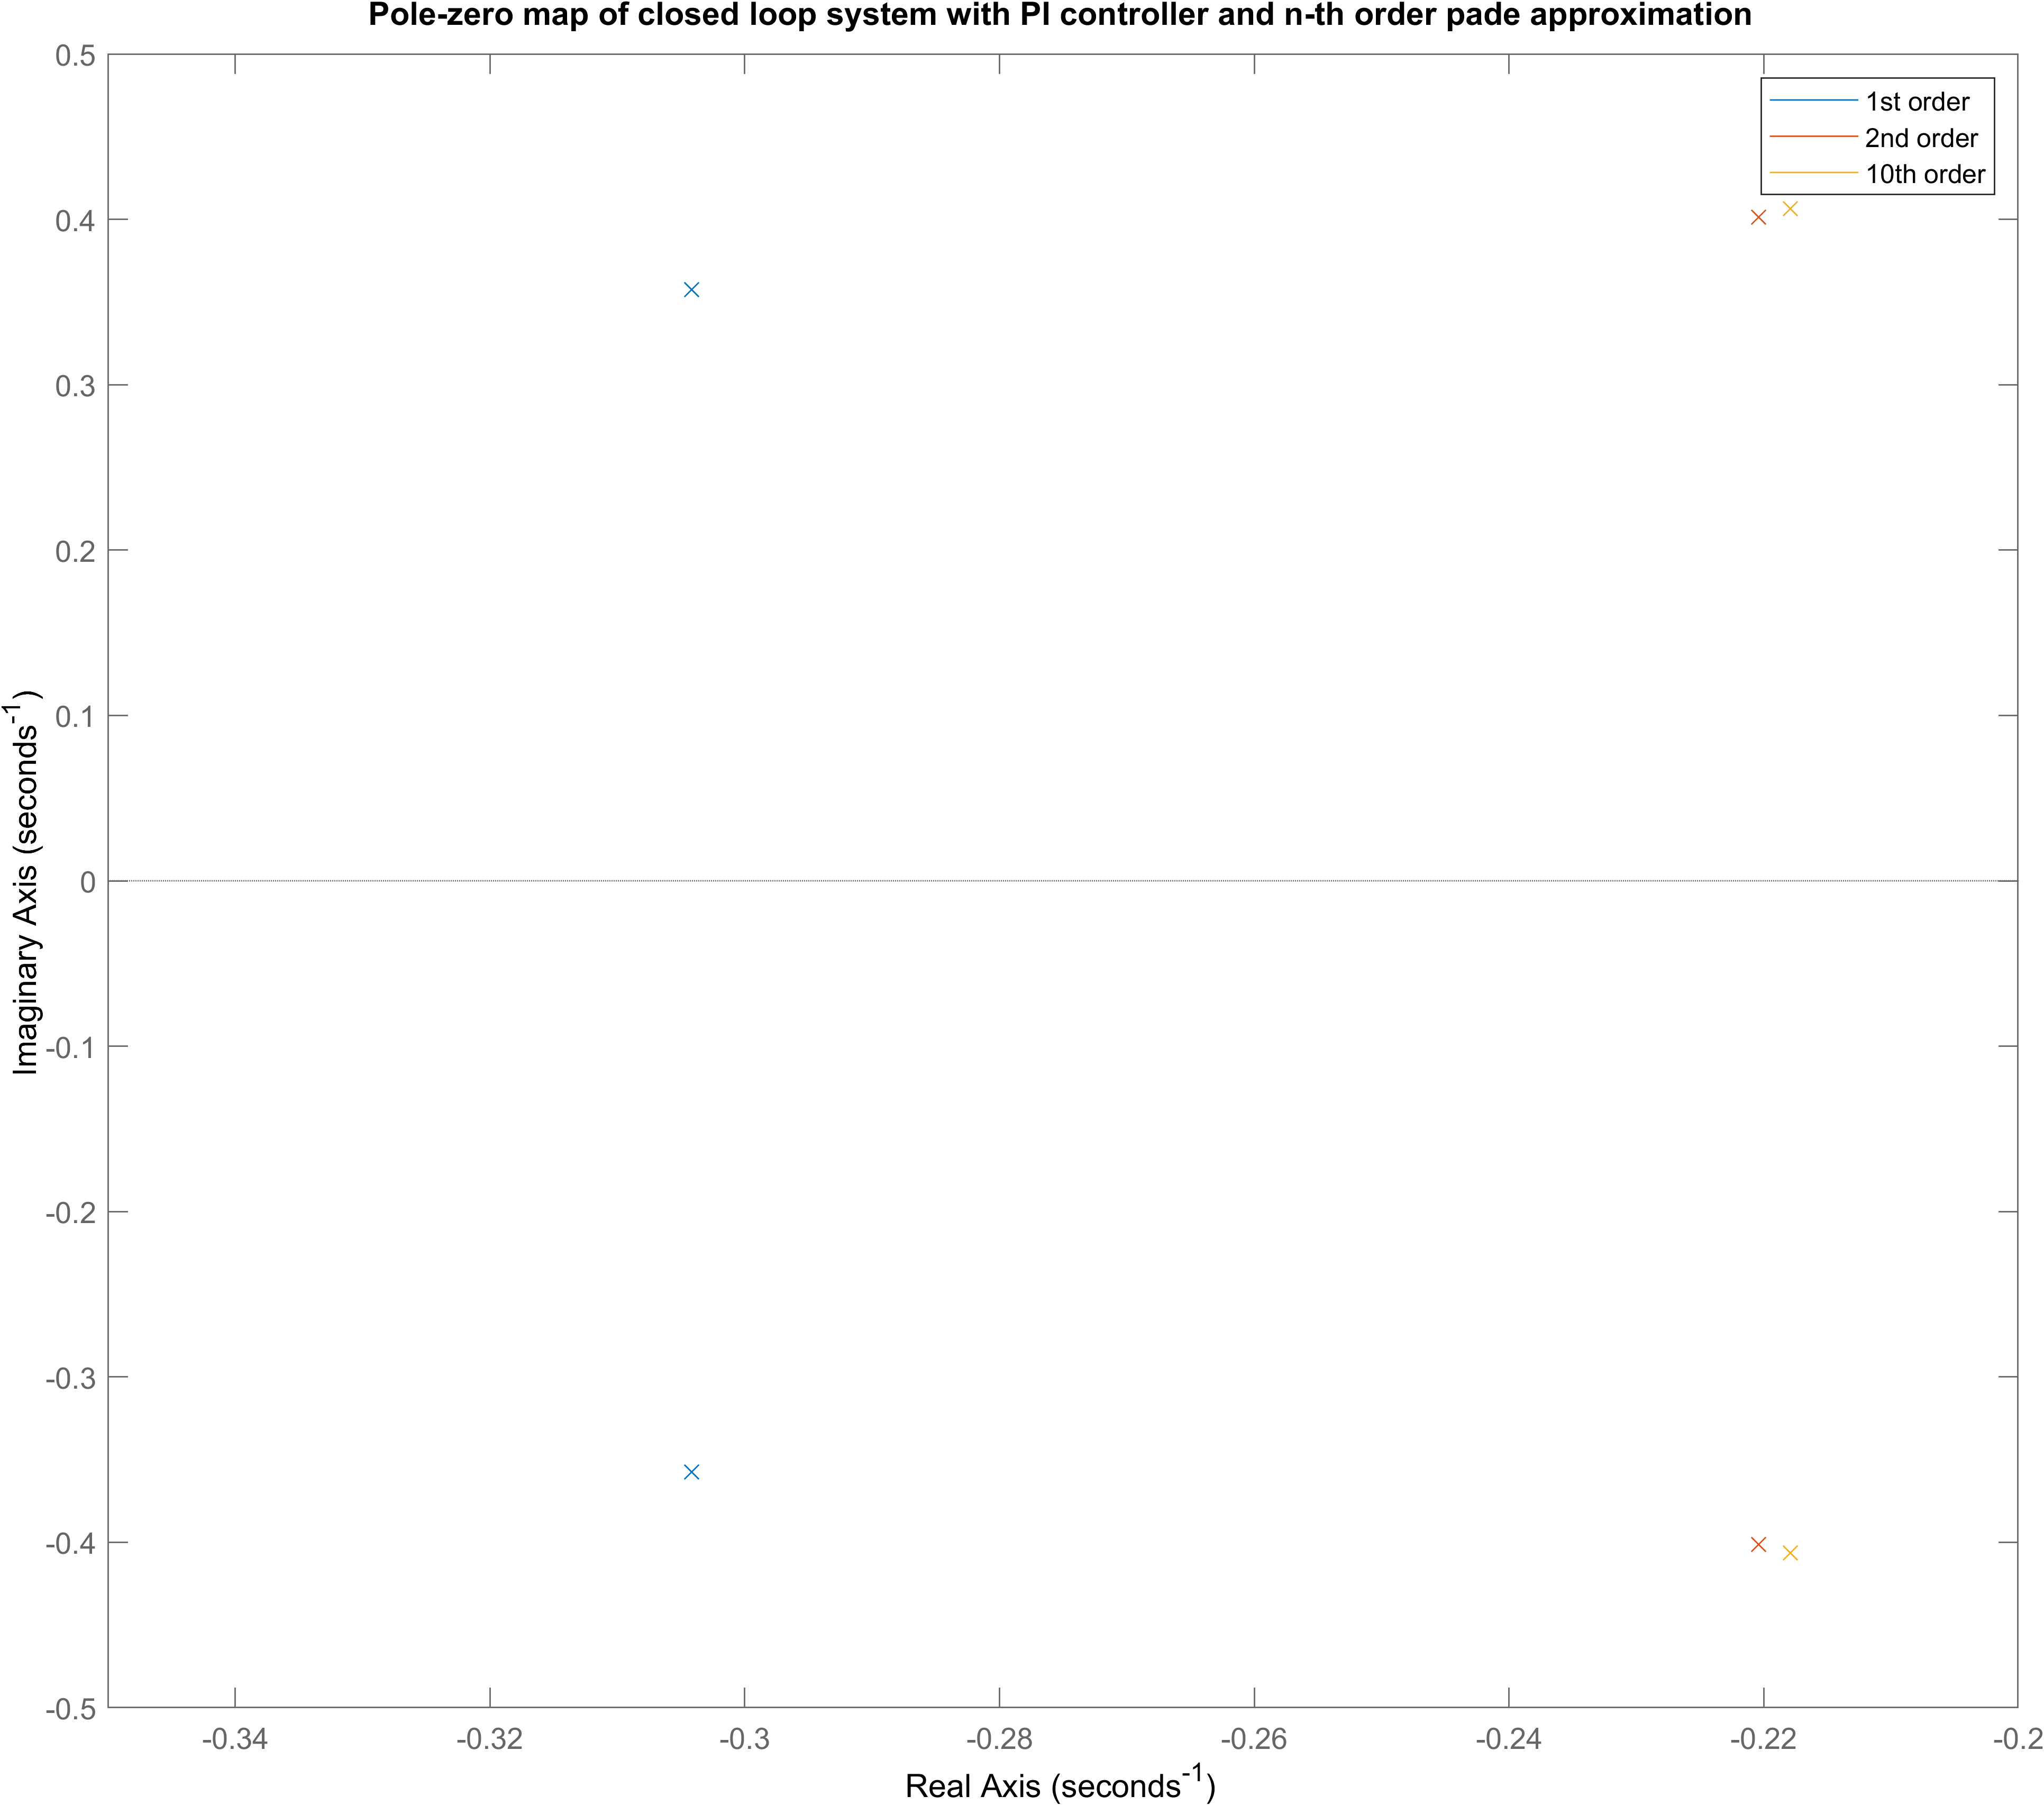
\includegraphics[height=5cm,width=0.5\linewidth]{Topics/ControlStructure/Graphics/PZmap_CL_zoom.png}
		\label{fig:PZmap_CL_zoom}
	\end{figure}
\end{frame}

\begin{frame}{Control Structure}{Control Requirements}
	Stability.\\
	Faster than outer loop.\\
	\hspace{0.3cm} - Bandwidth of $0.1 \frac{rad}{s}$ \\
	No steady state error.\\
	No overshoot, and low amount of oscillation.\\
\end{frame}

\begin{frame}{Control Structure}{Root Locus and Resulting Controller}
	\begin{figure}[h]
		\centering
		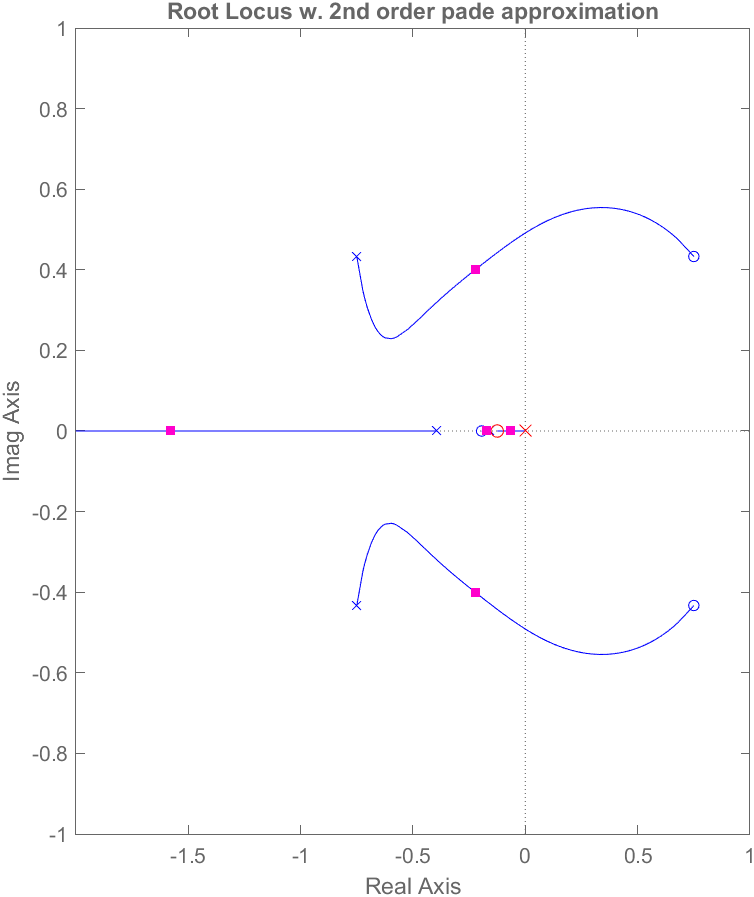
\includegraphics[height=4.8cm,width=0.48\linewidth]{Topics/ControlStructure/Graphics/RootLocus_Pade2.png}
		\label{fig:RootLocus}
	\end{figure}
	Results in controller transfer function:
	\begin{equation}\label{eq:PIDTransferFunction}
		C(s) = \frac{K_ps+K_i}{s} = \frac{1.8s+0.225}{s}
	\end{equation}
\end{frame}


\begin{frame}{Control Structure}{Step Response}
	\begin{figure}[h]
		\centering
		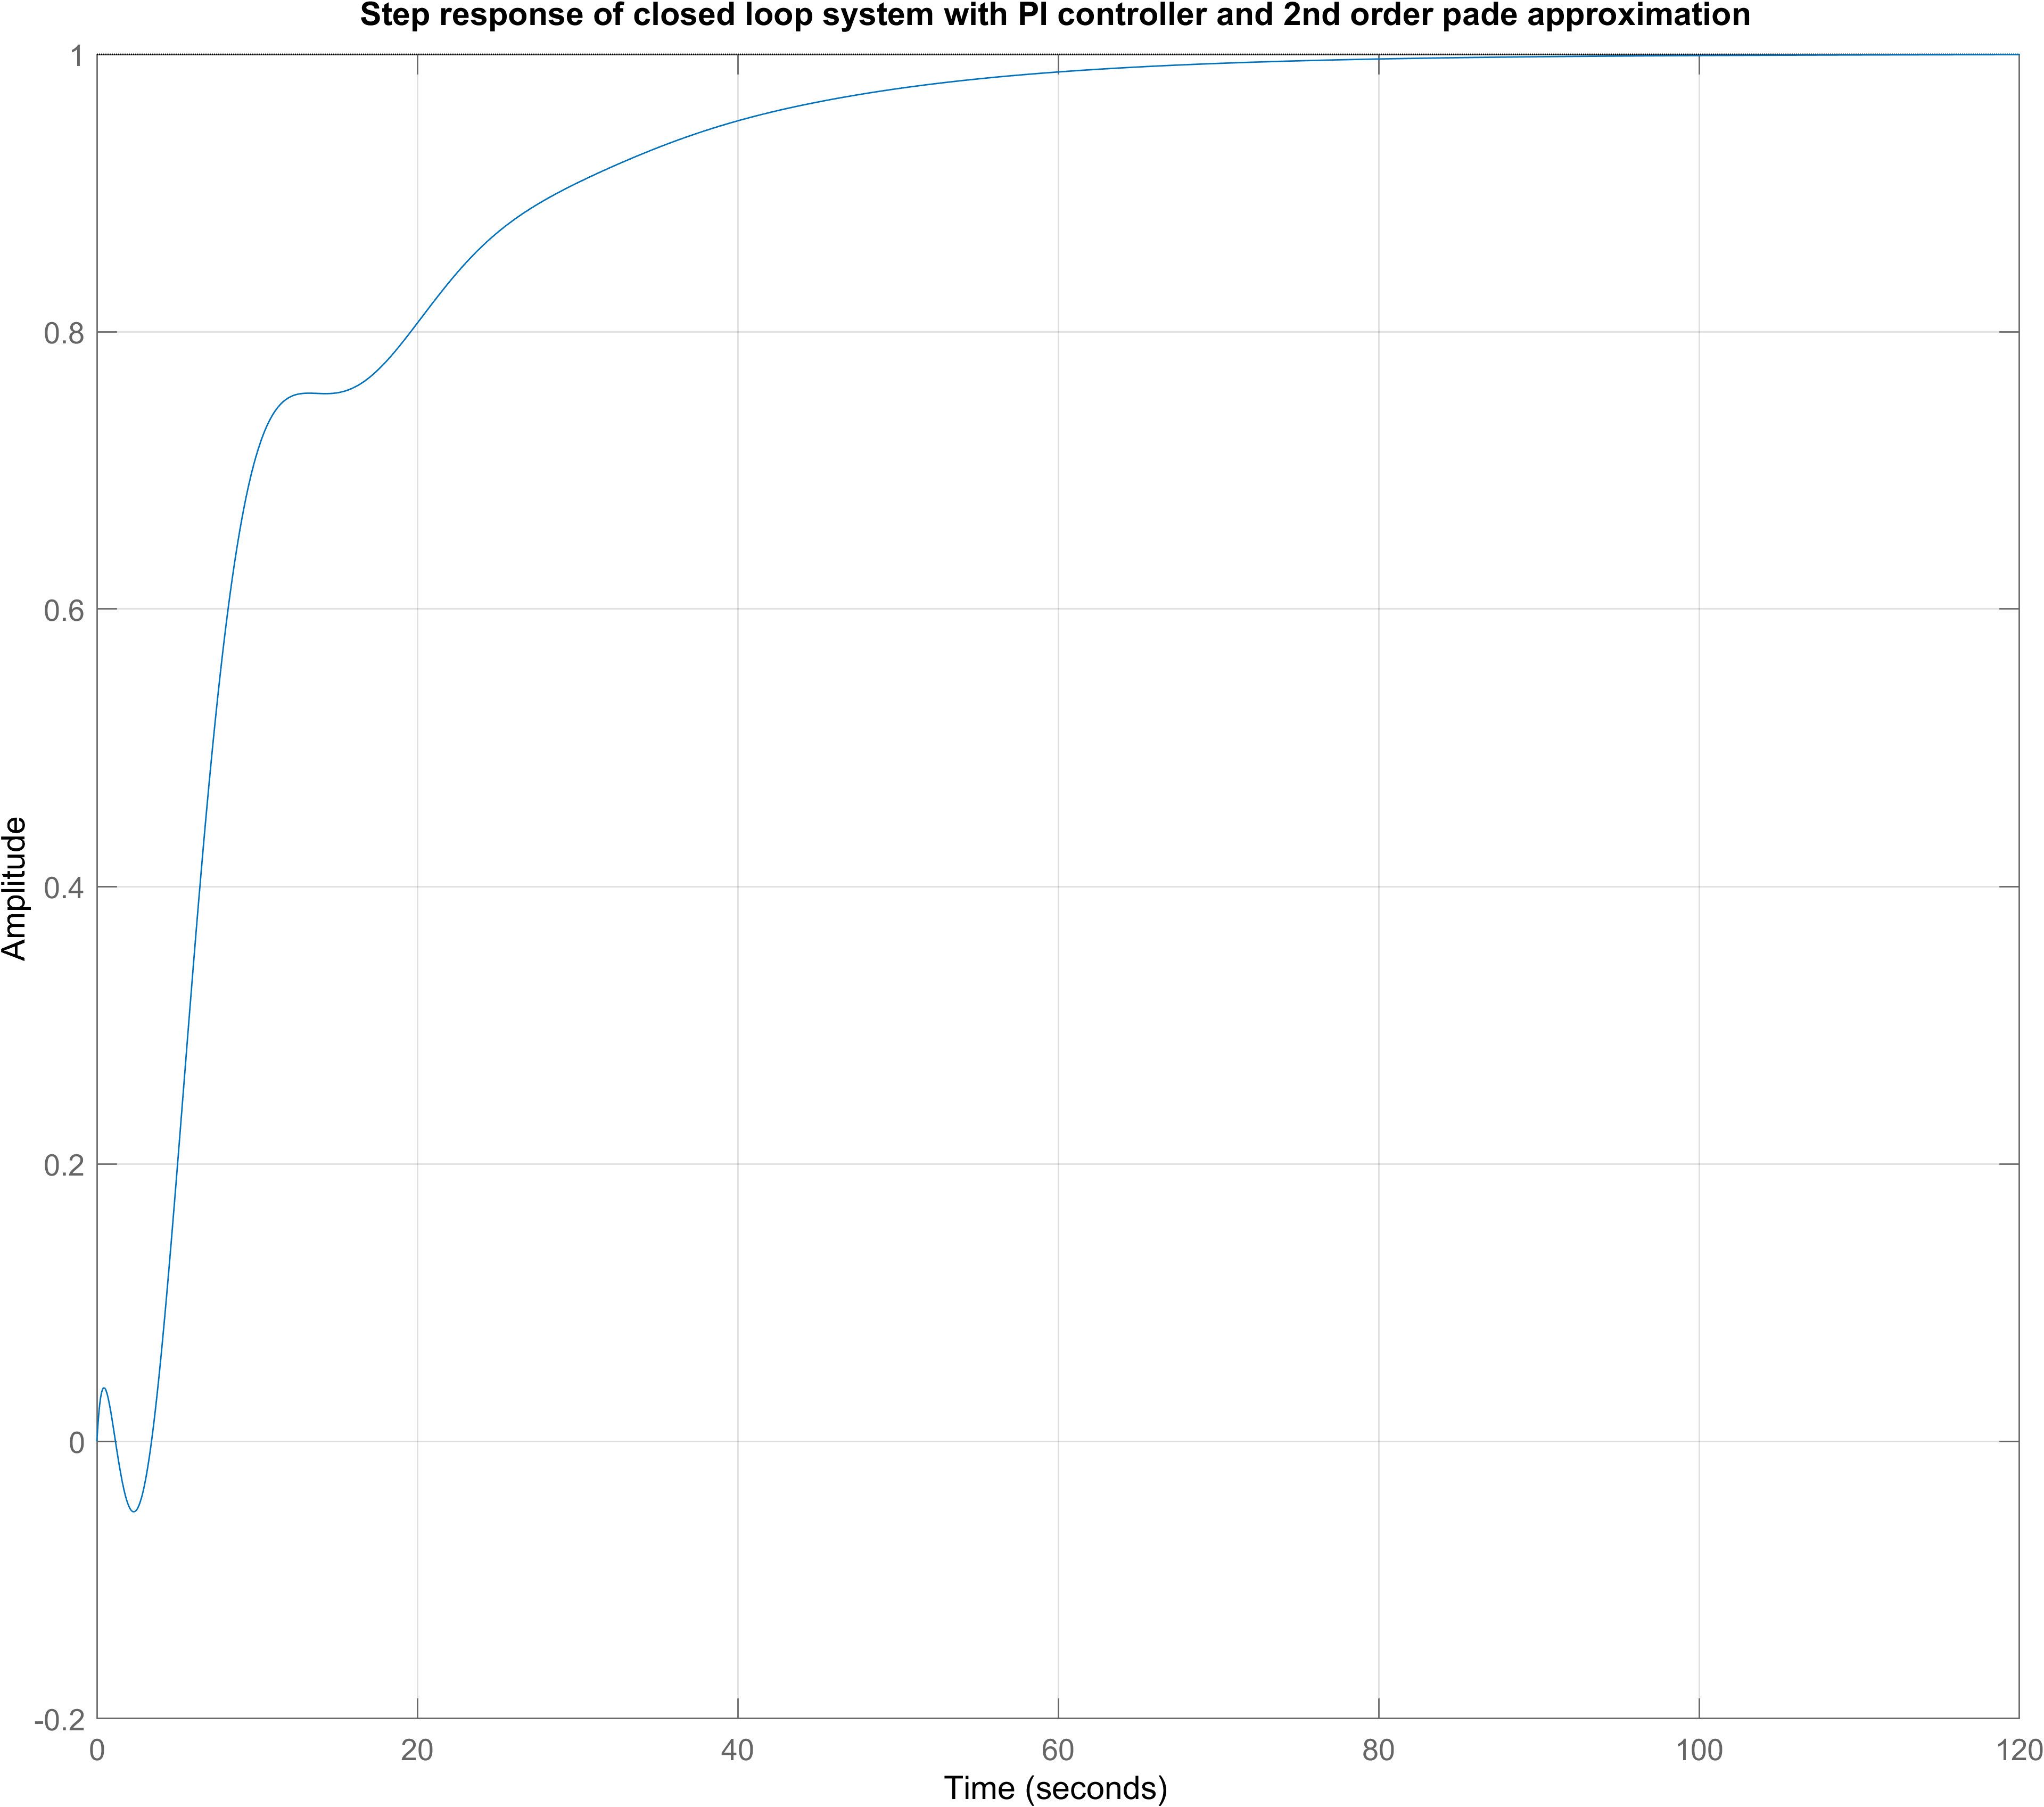
\includegraphics[height=6cm,width=0.6\linewidth]{Topics/ControlStructure/Graphics/StepResponse_Pade2.png}
		\label{fig:StepResponse_Pade2.png}
	\end{figure}

\end{frame}
